An astrophysical survey mapped all the galaxies in a small region of the sky, of angular diameter $\Delta \theta = \SI{0.01}{\radian}$, where many galaxies seemed to be concentrated around the central area of the image. When the positions and redshifts of all the galaxies in this cluster were measured, an interesting distribution emerged, which is shown in the plot below.

\begin{figure}[H]
    \centering
    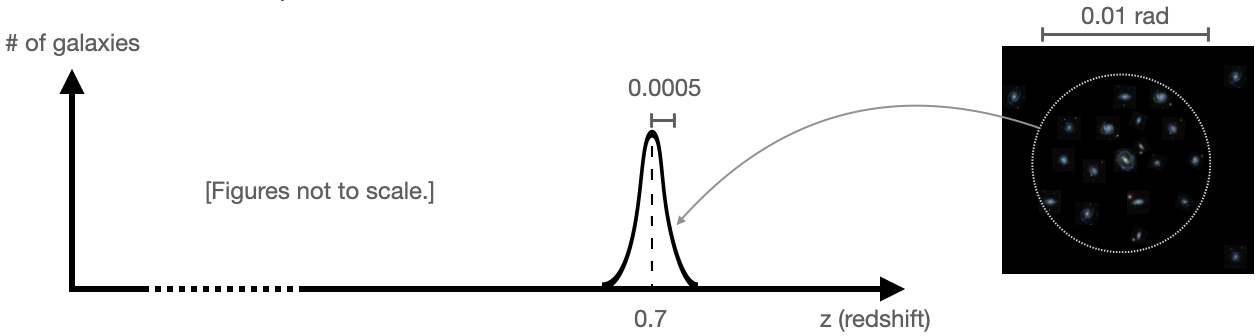
\includegraphics[width=1.0\textwidth]{2024/Theory/Figures/2024_TH_Q2_F1.png}
\end{figure}

Using these observations, estimate the total mass of the galaxy cluster and express your answer in solar masses. Assume that this galaxy cluster is in dynamical equilibrium, with a root-mean-square redshift dispersion $\sigma_z = \sqrt{\langle (z-0.7)^2 \rangle} = 0.0005$. Feel free to make reasonable approximations when considering the average velocities, masses, and spatial distribution of the galaxies.

Consider that the distance to $\bar z=0.7$ in the standard cosmological model is $D_A=1500\;\si{Mpc}$. Ignore cosmological effects on the distance.